\section{Suunnitelu}
Tarkoituksena oli tehdä sulautettu laite joka
\begin{itemize}
  \item voi ohjata LEDiä
  \item voidaan liittää verkkoon
  \item mahdollistaa LEDin ohjauksen verkkosivun kautta tai fyysistä nappia
    painamalla.
\end{itemize}
Vaatimuksena oli myös että piirilevy on itsetehty ja että siinä käytetään
mikrokontrolleria joka yhdistetään nettiin jonkunlaisen modeemin kautta
käyttäen AT-komentoja. Valitettavasti en itse ollut tietoinen tästä viimeisestä
vaatimuksesta, vaan ohjelmoin ESP8266 piirin suoraan. Tämän seurauksena
selostuksessa on puoli sivua ylimääräistä kohdassa~\ref{sec:extra}. Huomaamatta
jäi myös vaatimus fyysisestä painonapista, mutta sen lisääminen ei
onneksi ollut kovin iso työ.

Heti kun kuulin harjoitustyöstä halusin kokeilla käyttää ESP8266 moduulia
itsenäisesti ilman ohjaavaa mikrokontrolleria. Halusin myös ohjelmoida piirin
suoraan, enkä käyttää välissä käyttöjärjestelmää tai kolmannen osapuolen
firmwarea, kuten esimerkiksi NodeMcu:ta.\cite{nodemcu}

Syy tähän oli se että olin jo pitkään halunnut tutustua ESP8266 piiriin, mutten
ollut löytänyt sille aikaa. Halusin siis käyttää harkkatyön mahdollisimman
hyvin hyödyksi, ja uskoin että laitteistonläheinen C ja alustan tuomat
rajoitukset olisivat opettavaisia. Tykkään myös pyrkiä projekteissani
yksinkertaisuuteen aina kun se on mahdollista ja/tai järkevää.

Halusin myös tehdä mahdollisimman uudelleenkäytettävän piirilevyn, jotta sen
hyödyllisyys ei rajoittuisi tähän kurssiin.

\section{Piirilevy ja komponentit}
Päädyin käyttämään työssäni ESP-12E moduulia oikeastaan siitä syystä että sain
ostettua sellaisen lähipiiristäni. Oikeitakin syitä tämän moduulin
valitsemiselle kuitenkin on. Siinä on aikaisempia malleja enemmän liitäntöjä
piiriin (SPI ja 2 GPIO:ta lisää), piirillä on RF-häiriöitä vähentävä suojakuori
ja piirille on kuparivedoilla tehty pieni antenni, joka ainakin periaatteessa
parantaa moduuliin lähetys- ja vastaanottotehoja. Täytyy kuitenkin lisätä tähän
että loppujen lopuksi ainakin useimmissa harraste- ja kurssiprojekteissa eri
moduulien välillä ei ole huomattavia eroja.

Koska en käyttänyt työssäni erillistä mikrokontrolleria, jäi piirilevyni
erittäin yksinkertaiseksi. Itse jakaisin suunnittelemani piirin toiminnoiltaan
kolmeen osaan:
\begin{itemize}
  \item Moduulin liitäntöjen tarjoaminen piikkirimoilla
  \item Nappi resetointia varten ja kytkin piirin boottaustilan vaihtamiseksi
    flash-ohjelmoinnin ja flashista boottamisen välillä
  \item Virransyöttö
\end{itemize}

Koska itse halusin tehdä piirilevyn jota voisin käyttää myös kurssin jälkeen,
oli suhteellisen tärkeää että mahdollisimman moniin moduulin liitännöistä
pääsisi kätevästi käsiksi. Pinnirimoja on 3:
\begin{itemize}
  \item UART yhteyteen tarvittavat liitännät (mukaanlukien maa ja +3.3V ja +5V
    jännitteet)
  \item GPIO:t
  \item SPI liitännät
\end{itemize}

Omassa piirissäni on kytkin toimintatilan vaihtamiseen ja reset-nappi.
ESP8266 piirin toimintatila määräytyy sen perusteella missä jännitteessä
(maassa vai käyttöjännitteessä) tietyt piirin liitännät ovat. Tässä
harjoitustyössä ja useimissa projekteissa relevantit tilat ovat flash-muistin
ohjelmointitila ja flash-muistiin ohjelmoidun ohjelman ajaminen (boot from
flash). Kuvassa~\ref{fig:esp-tila-pinnit} on esitetty kyseiset liitännät ja
niiden kytkennät.
\begin{figure}[H]
  \centering
  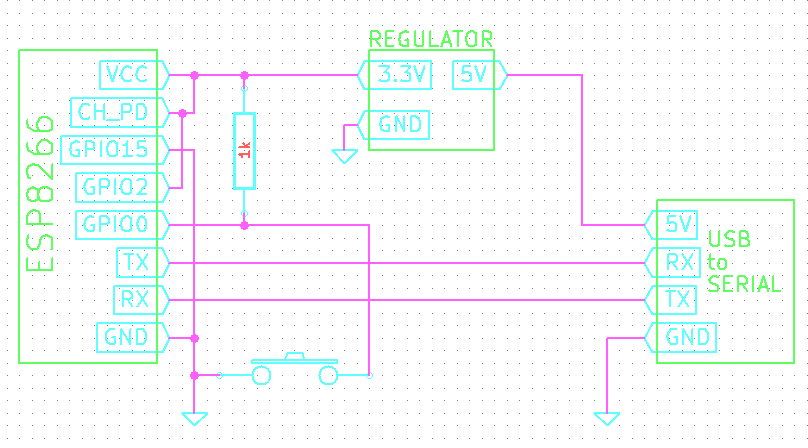
\includegraphics[width=0.8\linewidth]{esp-mode-setup}
  \caption{Kytkentä jossa napilla voidaan valita ohjelmoinnin ja boot-from-flash:n
    välillä~\cite{hackaday}}
\label{fig:esp-tila-pinnit}
\end{figure}

Virtalähteenä piirissäni on 9V paristo. Valitsin tämän pariston koska siihen
löytyy yksinkertainen ja yleinen liitäntä, ja koska +9V saa helposti laskettua
haluttuun +3.3V (ja +5V) jännitteeseen, jolloin tarvetta vaikkapa hakkurille
tai useammlle paristolle ei ole. Jännitteen reguloinnissa on käytetty LM317T
säädettävää lineaariregulaattoria. Regulaattorin ulos- ja sisääntulossa on
\(1\mu{}F\) kondensaattori ja lisäksi ESP-12 moduulin virtapinnien vieressä on
\(33\mu{}F\) kondensaattori (joka lienee hieman ylimitoitettu).

Kuvassa~\ref{fig:piiri-etu} on kuva piirilevyn etupuolesta, jossa näkyy hyvin
virransyötön komponentit (konkat, regulaattori ja paristoliitäntä) ja
piikkirimat. Vasemmalla ylhäällä on UART:tiin tarvitta piikkirima, sen
alapuolella SPI rima ja oikealla GPIO rima. Kuvassa~\ref{fig:piiri-taka} on
piirilevyn toinen puoli. Tällä puolella on itse ESP moduuli, reset-nappi ja
boottaustilan muuttava kytkin. Kuvassa~\ref{fig:nappi-ja-paristo} on piirilevyn
etupuoli ja LEDin tilaa muuttava ad-hoc painonappi ja teholähteenä toimiva
paristo.
\begin{figure}[H]
\centering
\begin{minipage}{.5\textwidth}
  \centering
  \includegraphics[width=0.9\linewidth]{front}
  \caption{Piirilevyn etupuoli}
\label{fig:piiri-etu}
\end{minipage}%
\begin{minipage}{.5\textwidth}
  \centering
  \includegraphics[width=0.9\linewidth]{back}
  \caption{Piirilevyn takapuoli}
\label{fig:piiri-taka}
\end{minipage}
\end{figure}
\begin{figure}[H]
  \centering
  \includegraphics[width=0.8\linewidth]{nappi-ja-paristo}
  \caption{}
\label{fig:nappi-ja-paristo}
\end{figure}

\section{Ohjelmisto}

\section{ESP8266 moduulin käyttäminen ilman mikrokontrolleria}
\label{sec:extra}

\section{Yhteenveto}

Projektin aikana törmäsin kuitenkin pariin suunnitteluvirheeseen:
\begin{itemize}
  \item Pienellä vaivalla olisin voinut lisätä piirille USB-to-UART piirin ja
    USB liittimen, joka olisi tehnyt ohjelmoinnista todella paljon helpompaa.
    Lisää tästä kohdassa~\ref{sec:extra}
\end{itemize}
